\subsection{Validation Results}
	Using the parameters set out in Table~\ref{tb:inputs_val} and the model we adapted, we were able to compare the temperature of our simulation against the temperature profile measured inside the CBHE during the TRT process. 
\subsection{Measurements and results from TRT}
	We were able to determine the corresponding thermal conductivity through the conventional TRT results. The undisturbed ground temperature 
	\begin{figure}[h!]
	\centering
	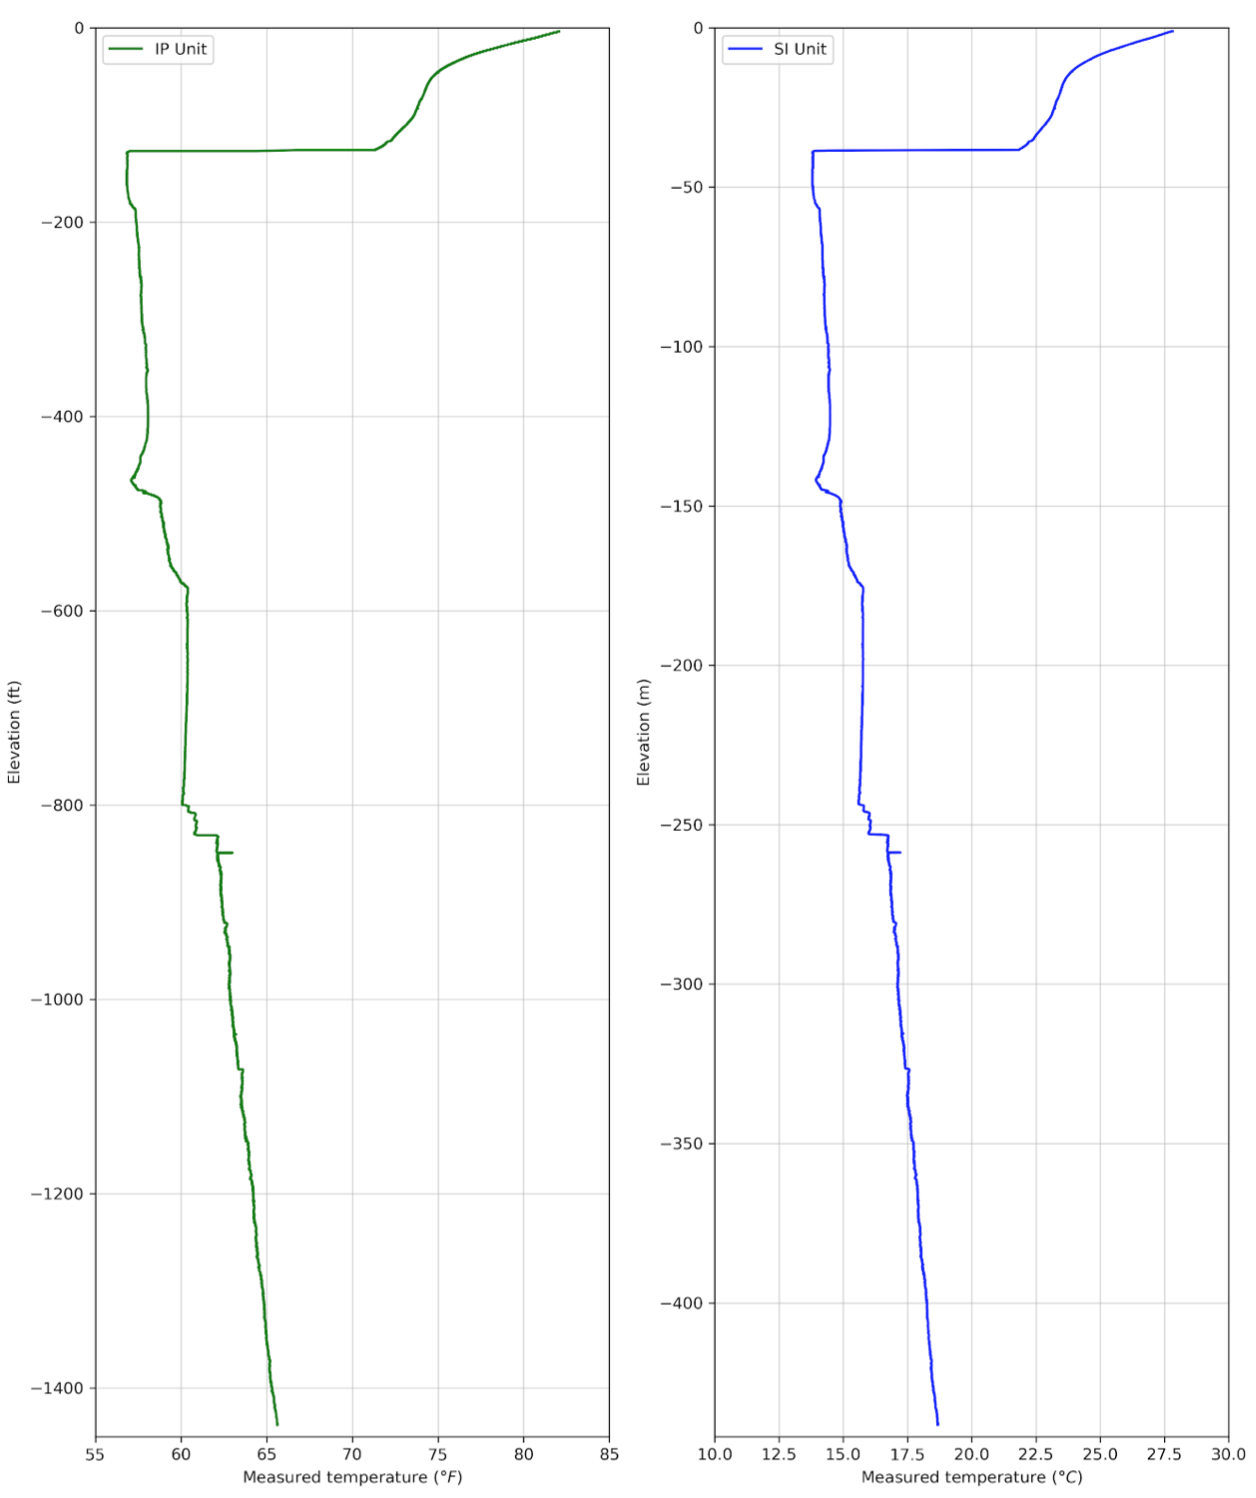
\includegraphics[height=0.5\textwidth]{data/groudref}
	\caption{Temperature measurement from fiber optic cable attached to the outside of CBHE at test site prior to the commencement of TRT.}	
	\end{figure}


\subsection{Parametric Study of other CBHE configuration}
	We're interested in improving the thermal performance of the borehole heat exchanger, particularly with respect to the designed and site-specific variables. 
	\subsubsection{Depth}
	
	\subsubsection{Site-specific variables}
	For site-specific variables, we examined the geothermal gradient and the thermal conductivity of potential sites. 
	
	%Also compare different Rb? Would this be an interesting thing to compare? I'd think so I hope??? Just generate a bunch of Rb and compre them.
	Ultimately, we compared the resulting $R_b$ of all the cases we investigated and plot them as a scattered plot to indicate the range of variations that may result in performance differences between different CBHEs. 
	